% Options for packages loaded elsewhere
\PassOptionsToPackage{unicode}{hyperref}
\PassOptionsToPackage{hyphens}{url}
\documentclass[
  10pt,
  a4paper,
]{article}
\usepackage{xcolor}
\usepackage[margin=22mm]{geometry}
\usepackage{amsmath,amssymb}
\setcounter{secnumdepth}{-\maxdimen} % remove section numbering
\usepackage{iftex}
\ifPDFTeX
  \usepackage[T1]{fontenc}
  \usepackage[utf8]{inputenc}
  \usepackage{textcomp} % provide euro and other symbols
\else % if luatex or xetex
  \usepackage{unicode-math} % this also loads fontspec
  \defaultfontfeatures{Scale=MatchLowercase}
  \defaultfontfeatures[\rmfamily]{Ligatures=TeX,Scale=1}
\fi
\usepackage{lmodern}
\ifPDFTeX\else
  % xetex/luatex font selection
\fi
% Use upquote if available, for straight quotes in verbatim environments
\IfFileExists{upquote.sty}{\usepackage{upquote}}{}
\IfFileExists{microtype.sty}{% use microtype if available
  \usepackage[]{microtype}
  \UseMicrotypeSet[protrusion]{basicmath} % disable protrusion for tt fonts
}{}
\makeatletter
\@ifundefined{KOMAClassName}{% if non-KOMA class
  \IfFileExists{parskip.sty}{%
    \usepackage{parskip}
  }{% else
    \setlength{\parindent}{0pt}
    \setlength{\parskip}{6pt plus 2pt minus 1pt}}
}{% if KOMA class
  \KOMAoptions{parskip=half}}
\makeatother
\usepackage{graphicx}
\makeatletter
\newsavebox\pandoc@box
\newcommand*\pandocbounded[1]{% scales image to fit in text height/width
  \sbox\pandoc@box{#1}%
  \Gscale@div\@tempa{\textheight}{\dimexpr\ht\pandoc@box+\dp\pandoc@box\relax}%
  \Gscale@div\@tempb{\linewidth}{\wd\pandoc@box}%
  \ifdim\@tempb\p@<\@tempa\p@\let\@tempa\@tempb\fi% select the smaller of both
  \ifdim\@tempa\p@<\p@\scalebox{\@tempa}{\usebox\pandoc@box}%
  \else\usebox{\pandoc@box}%
  \fi%
}
% Set default figure placement to htbp
\def\fps@figure{htbp}
\makeatother
\setlength{\emergencystretch}{3em} % prevent overfull lines
\providecommand{\tightlist}{%
  \setlength{\itemsep}{0pt}\setlength{\parskip}{0pt}}
\usepackage{mathrsfs}
\usepackage{mathtools}
\usepackage{xurl}
\emergencystretch=3em
\setcounter{tocdepth}{1}
\newcommand{\Beta}{\mathrm{B}}
\DeclareUnicodeCharacter{00B2}{\ensuremath{^2}}
\DeclareUnicodeCharacter{00B1}{\ensuremath{\pm}}
\DeclareUnicodeCharacter{00D7}{\ensuremath{\times}}
\DeclareUnicodeCharacter{2192}{\ensuremath{\to}}
\DeclareUnicodeCharacter{21D2}{\ensuremath{\Rightarrow}}
\DeclareUnicodeCharacter{21A6}{\ensuremath{\mapsto}}
\DeclareUnicodeCharacter{2208}{\ensuremath{\in}}
\DeclareUnicodeCharacter{2209}{\ensuremath{\notin}}
\DeclareUnicodeCharacter{2212}{\ensuremath{-}}
\DeclareUnicodeCharacter{2227}{\ensuremath{\wedge}}
\DeclareUnicodeCharacter{2228}{\ensuremath{\vee}}
\DeclareUnicodeCharacter{2260}{\ensuremath{\ne}}
\DeclareUnicodeCharacter{2264}{\ensuremath{\le}}
\DeclareUnicodeCharacter{2265}{\ensuremath{\ge}}
\DeclareUnicodeCharacter{2297}{\ensuremath{\otimes}}
\DeclareUnicodeCharacter{00B3}{\ensuremath{^3}}
\DeclareUnicodeCharacter{2074}{\ensuremath{^4}}
\DeclareUnicodeCharacter{2076}{\ensuremath{^6}}
\DeclareUnicodeCharacter{03BB}{\ensuremath{\lambda}}
\DeclareUnicodeCharacter{03BC}{\ensuremath{\mu}}
\DeclareUnicodeCharacter{03B5}{\ensuremath{\epsilon}}
\DeclareUnicodeCharacter{03C4}{\ensuremath{\tau}}
\DeclareUnicodeCharacter{03A6}{\ensuremath{\Phi}}
\DeclareUnicodeCharacter{03B1}{\ensuremath{\alpha}}
\DeclareUnicodeCharacter{03C3}{\ensuremath{\sigma}}
\DeclareUnicodeCharacter{03B4}{\ensuremath{\delta}}
\DeclareUnicodeCharacter{03C0}{\ensuremath{\pi}}
\DeclareUnicodeCharacter{039B}{\ensuremath{\Lambda}}
\DeclareUnicodeCharacter{2202}{\ensuremath{\partial}}
\DeclareUnicodeCharacter{0393}{\ensuremath{\Gamma}}
\DeclareUnicodeCharacter{2205}{\ensuremath{\varnothing}}
\DeclareUnicodeCharacter{221E}{\ensuremath{\infty}}
\DeclareUnicodeCharacter{2200}{\ensuremath{\forall}}
\DeclareUnicodeCharacter{00B9}{\ensuremath{^1}}
\DeclareUnicodeCharacter{00B0}{\ensuremath{{}^\circ}}
\DeclareUnicodeCharacter{211D}{\ensuremath{\mathbb{R}}}
\usepackage{bookmark}
\IfFileExists{xurl.sty}{\usepackage{xurl}}{} % add URL line breaks if available
\urlstyle{same}
\hypersetup{
  hidelinks,
  pdfcreator={LaTeX via pandoc}}

\author{}
\date{}

\begin{document}

{
\setcounter{tocdepth}{3}
\tableofcontents
}
\section{A proved bound over the complete first prime
window}\label{a-proved-bound-over-the-complete-first-prime-window}

\textbf{Original-zeta receiving calculation.} The working meromorphic
function is the original Riemann zeta, with its full Gamma/endpoints
multiplier and its full trivial-zero and pole divisor retained.
\href{FAITHFUL_THETA_COMPLETION_RETURN.md}{TF1--42} proves the original
labelled theta inverse and the actual heat-image defect.
\href{FAITHFUL_UNCOMPLETED_ZETA_HEAT.md}{UZ1--53} proves every
exceptional-point fibre, jet, original-zeta heat term and reflection
orientation.
\href{ORIGINAL_ZETA_COMPACT_WEIL_RECONSTRUCTION.md}{OZC1--48} rederives
the compact contour and interval operator directly from zeta, including
the left-cutoff Gamma boundary, and specifies exactly which compensated
pairing the bounds concern.
\href{ORIGINAL_ZETA_HEAT_CONTACT_RECONSTRUCTION.md}{OZH1--49} rederives
the actual meromorphic heat, rational signed trace, compact-test domain,
contact drift and full causal arithmetic variation. The raw full divisor
and the compensated Weil receiver are linked by their displayed
correction, not identified. In particular the fixed-test trivial-zero
sum converges exactly at translations at least 1/32 and equals the
earlier R term; at zero translation it requires the proved cutoff
compensation. \href{ORIGINAL_ZETA_CAUCHY_RECONSTRUCTION.md}{OZK1--38}
reconstructs the original signed Cauchy trace, its full Gamma
correction, resonant finite parts, every finite matrix and its index,
and the complete local heat jets. Its invertible map retains the raw
trace and correction separately. These complete receiving proofs govern
the interpretation of the retained auxiliary calculations below.

This calculation applies the full compact-interval estimate to the
original fixed test of UP and PW. It proves the required
translated-correlation bound on a specified interval containing the
whole contribution of prime two, with a strict margin. It retains the
negative archimedean cross term and both signs of the two-test Weil
form. The calculation does not extend its proved interval to arbitrary
translations.

\subsection{1. Original test, form, and exact local
estimate}\label{original-test-form-and-exact-local-estimate}

Retain the original conventions \[
M_f(s)=\int_{\mathbb R}f(v)e^{-(s-1/2)v}\,dv,\qquad
f^\#(v)=\overline{f(-v)},\qquad
T=\partial_v^2-\tfrac14,
\tag{FW1}
\] and the complete original pairing \[
B(f,g)=\sum_\rho m_\rho\overline{M_f(1-\bar\rho)}M_g(\rho),
\qquad Q(f)=B(f,f).
\tag{FW2}
\] The zeros are the actual nontrivial zeta zeros with their actual
multiplicities. The absolute convergence and the complete supported
explicit formula are proved in PW1--2 and SZW24--38. No endpoint is
removed without evaluating its moment.

Use exactly the fixed density and test \[
\begin{gathered}
r=\tfrac1{64},\qquad
b_r=\mathop{*}_{j\ge1}\frac{\mathbf1_{[-r2^{-j},r2^{-j}]}}{2r2^{-j}},\qquad
f_r=Tb_r,\\
k_r=b_r*b_r,\qquad h_r=f_r*f_r=T^2k_r,\qquad
N_r=\|f_r\|_2^2>0.
\end{gathered}\tag{FW3}
\] Their full construction and Fourier product are retained in UP1--14
and PW3--5, including the classical compact bump attribution. The
functions are real, even and smooth, with supports of \(b_r,f_r\)
contained in \([-r,r]\) and those of \(k_r,h_r\) contained in
\([-2r,2r]\). Also \(k_r\ge0\), \(\int k_r=1\), and \(h_r(0)=N_r\).
Twice integrating by parts gives \(M_{f_r}(s)=s(s-1)G_r(s-1/2)\), so
both endpoint moments vanish exactly.

The complete proof \href{FIRST_PRIME_FULL_WEIL_COERCIVITY.md}{FC, full
first-prime interval coercivity} establishes, with all prime-two and
Gamma terms retained, \[
Q(F)>c_*\|F\|_2^2\quad(F\ne0),\qquad
c_*:=\frac{11509}{600000}>\frac1{64},\qquad
\operatorname{diam}(\operatorname{supp}F)\le T_*:=\frac{19}{25},
\tag{FW4}
\] for every compact smooth complex test satisfying \(M_F(0)=M_F(1)=0\).
For \(F=0\), the corresponding non-strict inequality is equality. The
source derives (FW4) from the full compact-interval operator, the exact
two moments, the boundary potential dominating the prime-two
translation, and a rational bound for its analytic remainder. This proof
uses that entire result, without imposing separate moment conditions on
pieces of a test.

Define the actual translated quantities \[
f_a(v)=f_r(v-a),\qquad
K(a)=B(f_a,f_r),\quad q=K(0),\quad
C(a)=\langle f_a,f_r\rangle_{L^2}=h_r(a),\quad
A_*:=T_*-2r=\frac{583}{800}.
\tag{FW5}
\] Here \(K\) is real and even by PW6--8, and \(B(f_a,f_b)=K(a-b)\),
while \(\langle f_a,f_b\rangle=C(a-b)\). These equalities follow by a
change of variable for Haar measure and cancellation of the two
translation exponentials in (FW2). The complete diagonal is \(q\),
unchanged by translation. In particular (FW4) on the single nonzero test
proves \(q>c_*N_r\).

\subsection{2. Every finite rank on the specified translation
interval}\label{every-finite-rank-on-the-specified-translation-interval}

Let \(a_1,\ldots,a_n\) be distinct real numbers with
\(\max a_j-\min a_j\le A_*\). For every coefficient vector
\(z\in\mathbb C^n\), set \[
F_z=\sum_{j=1}^n z_j f_{a_j}.
\tag{FW6}
\] Each summand has both endpoint moments zero: translation multiplies
those moments by \(e^{-(s-1/2)a_j}\), which leaves their zero values
unchanged. Hence \(F_z\) has the original two global moments zero. Its
support is contained in \([\min a_j-r,\max a_j+r]\), whose length is at
most \(T_*\).

For \(z\ne0\), this test is nonzero. To prove linear independence of
these actual translates, take the Fourier transform of a putative zero
relation. The transform of \(f_r\) is nonzero on an open real interval
because it is an entire function that is not identically zero. On that
interval the relation forces \(\sum z_j e^{-i a_j y}=0\). This entire
exponential polynomial is then identically zero. Its first \(n\)
derivatives at zero give the Vandermonde system with determinant
\(\prod_{i<j}(-ia_j+ia_i)\ne0\); all \(z_j\) vanish. This proves the
assertion for every finite distinct centre list.

Applying (FW4) to (FW6) and expanding both forms gives the exact matrix
inequality \[
\boxed{
[K(a_i-a_j)]_{i,j=1}^n
-c_*[h_r(a_i-a_j)]_{i,j=1}^n\succ0
\quad\text{when }\max a_j-\min a_j\le\frac{583}{800}.}
\tag{FW7}
\] It holds at every finite rank on this specified interval. Repeated
centres can instead be retained, giving the non-strict inequality and
the exact kernel of their coefficient-summing map. No finite-rank
conclusion is extrapolated to centre lists with larger diameter.

\subsection{3. The exact two-translate bound and its strict
margin}\label{the-exact-two-translate-bound-and-its-strict-margin}

For \(0<a\le A_*\), the two-by-two instance of (FW7) has diagonal
\(q-c_*N_r>0\) and real off-diagonal \(K(a)-c_*h_r(a)\). Its two
eigenvalues are the diagonal plus and minus that off-diagonal. Both are
positive. Therefore \[
\boxed{|K(a)-c_*h_r(a)|<q-c_*N_r\qquad(0<a\le583/800).}
\tag{FW8}
\] At \(a=0\) the corresponding inequality is equality. When
\(a\ge2r=1/32\), the two translated supports overlap at most at an
endpoint and \(h_r(a)=0\). Thus \[
\boxed{|K(a)|<q-c_*N_r<q
\qquad\left(\frac1{32}\le a\le\frac{583}{800}\right).}
\tag{FW9}
\] For \(0<a<2r\), Haar Cauchy--Schwarz gives \(|h_r(a)|\le N_r\), and
(FW8) also implies \(|K(a)|<q\). Consequently the original RH-equivalent
inequality is proved throughout \([0,583/800]\); its value at zero is
the stated equality. Its unproved part consists of larger translations.

In particular both original signed two-test values satisfy \[
Q(f_r+f_a)=2q+2K(a)>2c_*N_r,\qquad
Q(f_r-f_a)=2q-2K(a)>2c_*N_r
\tag{FW10}
\] on the interval in (FW9). Both tests retain their exact endpoint-zero
support carriers. The sign of their off-diagonal correlation has not
been substituted for the sign of either quadratic form.

\subsection{4. The whole prime-two contribution and the negative cross
term}\label{the-whole-prime-two-contribution-and-the-negative-cross-term}

Put \(L=\log2\) and \(\beta=L/\sqrt2\). The exact first prime window is
\[
I_2=[L-1/32,L+1/32].
\tag{FW11}
\] It lies strictly inside the interval in (FW9). Here is a rational
verification of the required endpoint comparison. The convergent
identity \(\log2=2\sum_{j\ge0}[(2j+1)3^{2j+1}]^{-1}\) follows by
integrating the geometric series for \((1-x^2)^{-1}\) from zero to
\(1/3\). Its first four terms give a lower bound greater than \(2/3\).
Bounding every denominator in the remaining tail below by nine gives \[
\log2\le
2\sum_{j=0}^{3}\frac1{(2j+1)3^{2j+1}}
+\frac1{4\cdot3^9}
<\frac{139}{200}.
\tag{FW12}
\] The last comparison is between rational numbers. Hence
\(L+1/16<139/200+1/16=303/400<19/25\), proving \(L+1/32<A_*\). The lower
window endpoint exceeds \(1/32\) because \(L>2/3>1/16\).

For every \(1/32<a\le A_*\), only the prime power two can occur in the
full PW13 sum: its largest possible index satisfies
\(\log n\le a+1/32\le19/25<1<\log3\), the last inequality following from
\(e<11/4<3\). All terms with indices at least three vanish through the
test support, with their labelled coordinates retained. The complete
correlation is therefore \[
\boxed{K(a)=-R_r(a)-\beta h_r(a-L),}
\qquad
R_r(a)=\int_{a-1/32}^{a+1/32}W(v)k_r(a-v)\,dv>0,
\tag{FW13}
\] where the unchanged explicit kernel is \[
W(v)=\frac{4e^{-5v/2}(9+55e^{-2v}+31e^{-4v}+e^{-6v})}
{(1-e^{-2v})^5},\qquad v>0.
\tag{FW14}
\] PW15--17 proves these identities by four integrations by parts with
the actual filter \(T^2\). Combining (FW9) and (FW13) proves the full
arithmetic estimate \[
\boxed{\left|R_r(a)+\frac{\log2}{\sqrt2}h_r(a-\log2)\right|
<q-\frac{11509}{600000}\|f_r\|_2^2
\quad\left(\frac1{32}<a\le\frac{583}{800}\right).}
\tag{FW15}
\] This covers the entire window \(I_2\), including the two endpoints
where the prime-two amplitude vanishes. The smaller-support terms have
not been compared separately by assigning them unproved signs.

At its centre the complete off-diagonal value and resulting diagonal
estimate are especially explicit: \[
K(\log2)=-R_r(\log2)-\frac{\log2}{\sqrt2}N_r<0,
\qquad
q>\left(\frac{\log2}{\sqrt2}+c_*\right)N_r+R_r(\log2).
\tag{FW16}
\] The inequality is exactly (FW15) with \(h_r(0)=N_r\). This strictly
negative cross term is compatible with the strict positivity of both
signed quadratic tests in (FW10); all four terms of their bilinear
expansion are retained.

\subsection{5. Original supported-zero maps and the remaining
translations}\label{original-supported-zero-maps-and-the-remaining-translations}

Let \(\mathscr L\) be the original nontrivial bounded distributive
support lattice. The linear map \(z\mapsto F_z\), each translation, the
moment map, and \(T\) have the exact fixed-carrier lift
\((x,\lambda)\mapsto(Ax,\lambda)\). Addition uses the original join, and
scalar multiplication uses the original meet. Direct substitution proves
additivity and scalar compatibility, as in UP34. The endpoint map sends
every top-labelled test in (FW6) to \((0,1_{\mathscr L})\), while the
unsupported input remains \((0,0_{\mathscr L})\). The zero endpoint
amplitude therefore retains supported zero \(e\ne\tau\).

The pairing lift is \[
B^{\mathscr L}((u,\lambda),(v,\mu))=(B(u,v),\lambda\wedge\mu).
\tag{FW17}
\] Its compatibility follows from sesquilinearity and distributivity. In
particular the finite Gram matrices in (FW7) are values of the existing
lifted form, not replacement support spaces. On the translated
convolution the original full formula has \[
\boldsymbol B_{\mathscr L}=0,\qquad
\boldsymbol Z_{\mathscr L}=K(a)\mathbf e_{1_{\mathscr L}},\qquad
\boldsymbol D_{\mathscr L}=-K(a)\mathbf e_{1_{\mathscr L}}.
\tag{FW18}
\] All lower coordinate functionals have their evaluated zero endpoint
amplitudes; their coordinate spaces and support labels persist. Formula
(FW13) is their top amplitude, with the actual prime-two coefficient and
entire archimedean term.

\subsection{6. Continue the two-test estimate across the following prime
gap}\label{continue-the-two-test-estimate-across-the-following-prime-gap}

The first estimate also supplies a bound on the next full gap, without
changing the fixed test. Put \[
A_3=\log3-2r=\log3-\frac1{32}.
\tag{FW19}
\] The exact inequalities already proved give \(\log2+2r<A_*<A_3\): the
left comparison is (FW12), and the right follows from \(\log3>1\) and
\(A_*<1-1/32\). For \(A_*\le a\le A_3\), prime two lies strictly below
the support window. Every \(n\ge3\) lies above it, except that \(n=3\)
meets its upper endpoint when \(a=A_3\). At that endpoint its value is
\(h_r(-2r)=0\), since \(h_r\) is smooth and supported in \([-2r,2r]\).
The complete finite-prime sum therefore vanishes on this closed
interval.

PW16 gives the absolutely convergent positive series, differentiable on
every compact subset of \(a>2r\), \[
R_r(a)=\sum_{j\ge1}4j^2(2j+1)^2
G_r(2j+1/2)^2e^{-(2j+1/2)a},\qquad R_r'(a)<0.
\tag{FW20}
\] Every coefficient is strictly positive because
\(G_r(x)=\int b_r(v)e^{-xv}\,dv>0\) on the real axis. Its growth bound
\(G_r(x)\le e^{r|x|}\) makes the differentiated series uniformly
convergent when \(a\) is bounded away from \(2r\). The full formula
consequently gives \(K(a)=-R_r(a)\) throughout this gap. At \(A_*\),
(FW9) gives \(R_r(A_*)<q-c_*N_r\). Monotonicity now proves \[
\boxed{|K(a)|<q-c_*N_r<q\qquad
\frac1{32}\le a\le\log3-\frac1{32}.}
\tag{FW21}
\] For the first part of this interval use (FW9); for its remaining part
use (FW20). Both inequalities (FW10) extend over the whole interval in
(FW21). Together with (FW8), this proves \(|K(a)|<q\) for every
\(0<a\le A_3\), and equality at \(a=0\). The every-rank matrix theorem
(FW7) retains its stated diameter \(583/800\); this prime-gap argument
extends the two-test bound and does not assert that larger matrix
theorem.

The full criterion PW20 still requires the inequality for
\(a>\log3-1/32\). The results here prove a strict margin on the complete
first-prime window, its following gap, and all finite centre
configurations of the stated smaller diameter. They do not establish the
remaining global inequality or infer RH from a finite interval.

\subsection{Sources and attribution}\label{sources-and-attribution}

The incoming programme note \emph{Direct RH continuation: the optimal
packet cost in the full Weil form}, dated 23 September 2026, supplied
the complete compact-interval operator and the rational
three-quarter-support estimate at N1--16 and N48--52. Its original
source SHA256 is
\texttt{d3b1ac08\allowbreak{}c71f6104\allowbreak{}cfe011ba\allowbreak{}5e5b86f6\allowbreak{}fbe18291\allowbreak{}6c0b0270\allowbreak{}511671b1\allowbreak{}f7165d5b};
it contains 84 equation tags in the N1--N60 and G1--G18 systems,
including suffixes. Root read that complete source. FC reproduces the
full mathematical ingredients used here, checks the incoming bound, and
proves its explicit extension to 19/25. The incoming author's
packet-cost claims are not needed for (FW1)--(FW18). The precise
application to the unchanged UP/PW test, every-rank local Gram, strict
correlation margin, whole first-prime window, and supported maps is
proved above. The complete original programme dependencies accompany
this edition, with their human citations and classical compact-bump
attribution retained.

\subsection{Exact objects and proved
bounds}\label{exact-objects-and-proved-bounds}

\begin{figure}
\centering
\pandocbounded{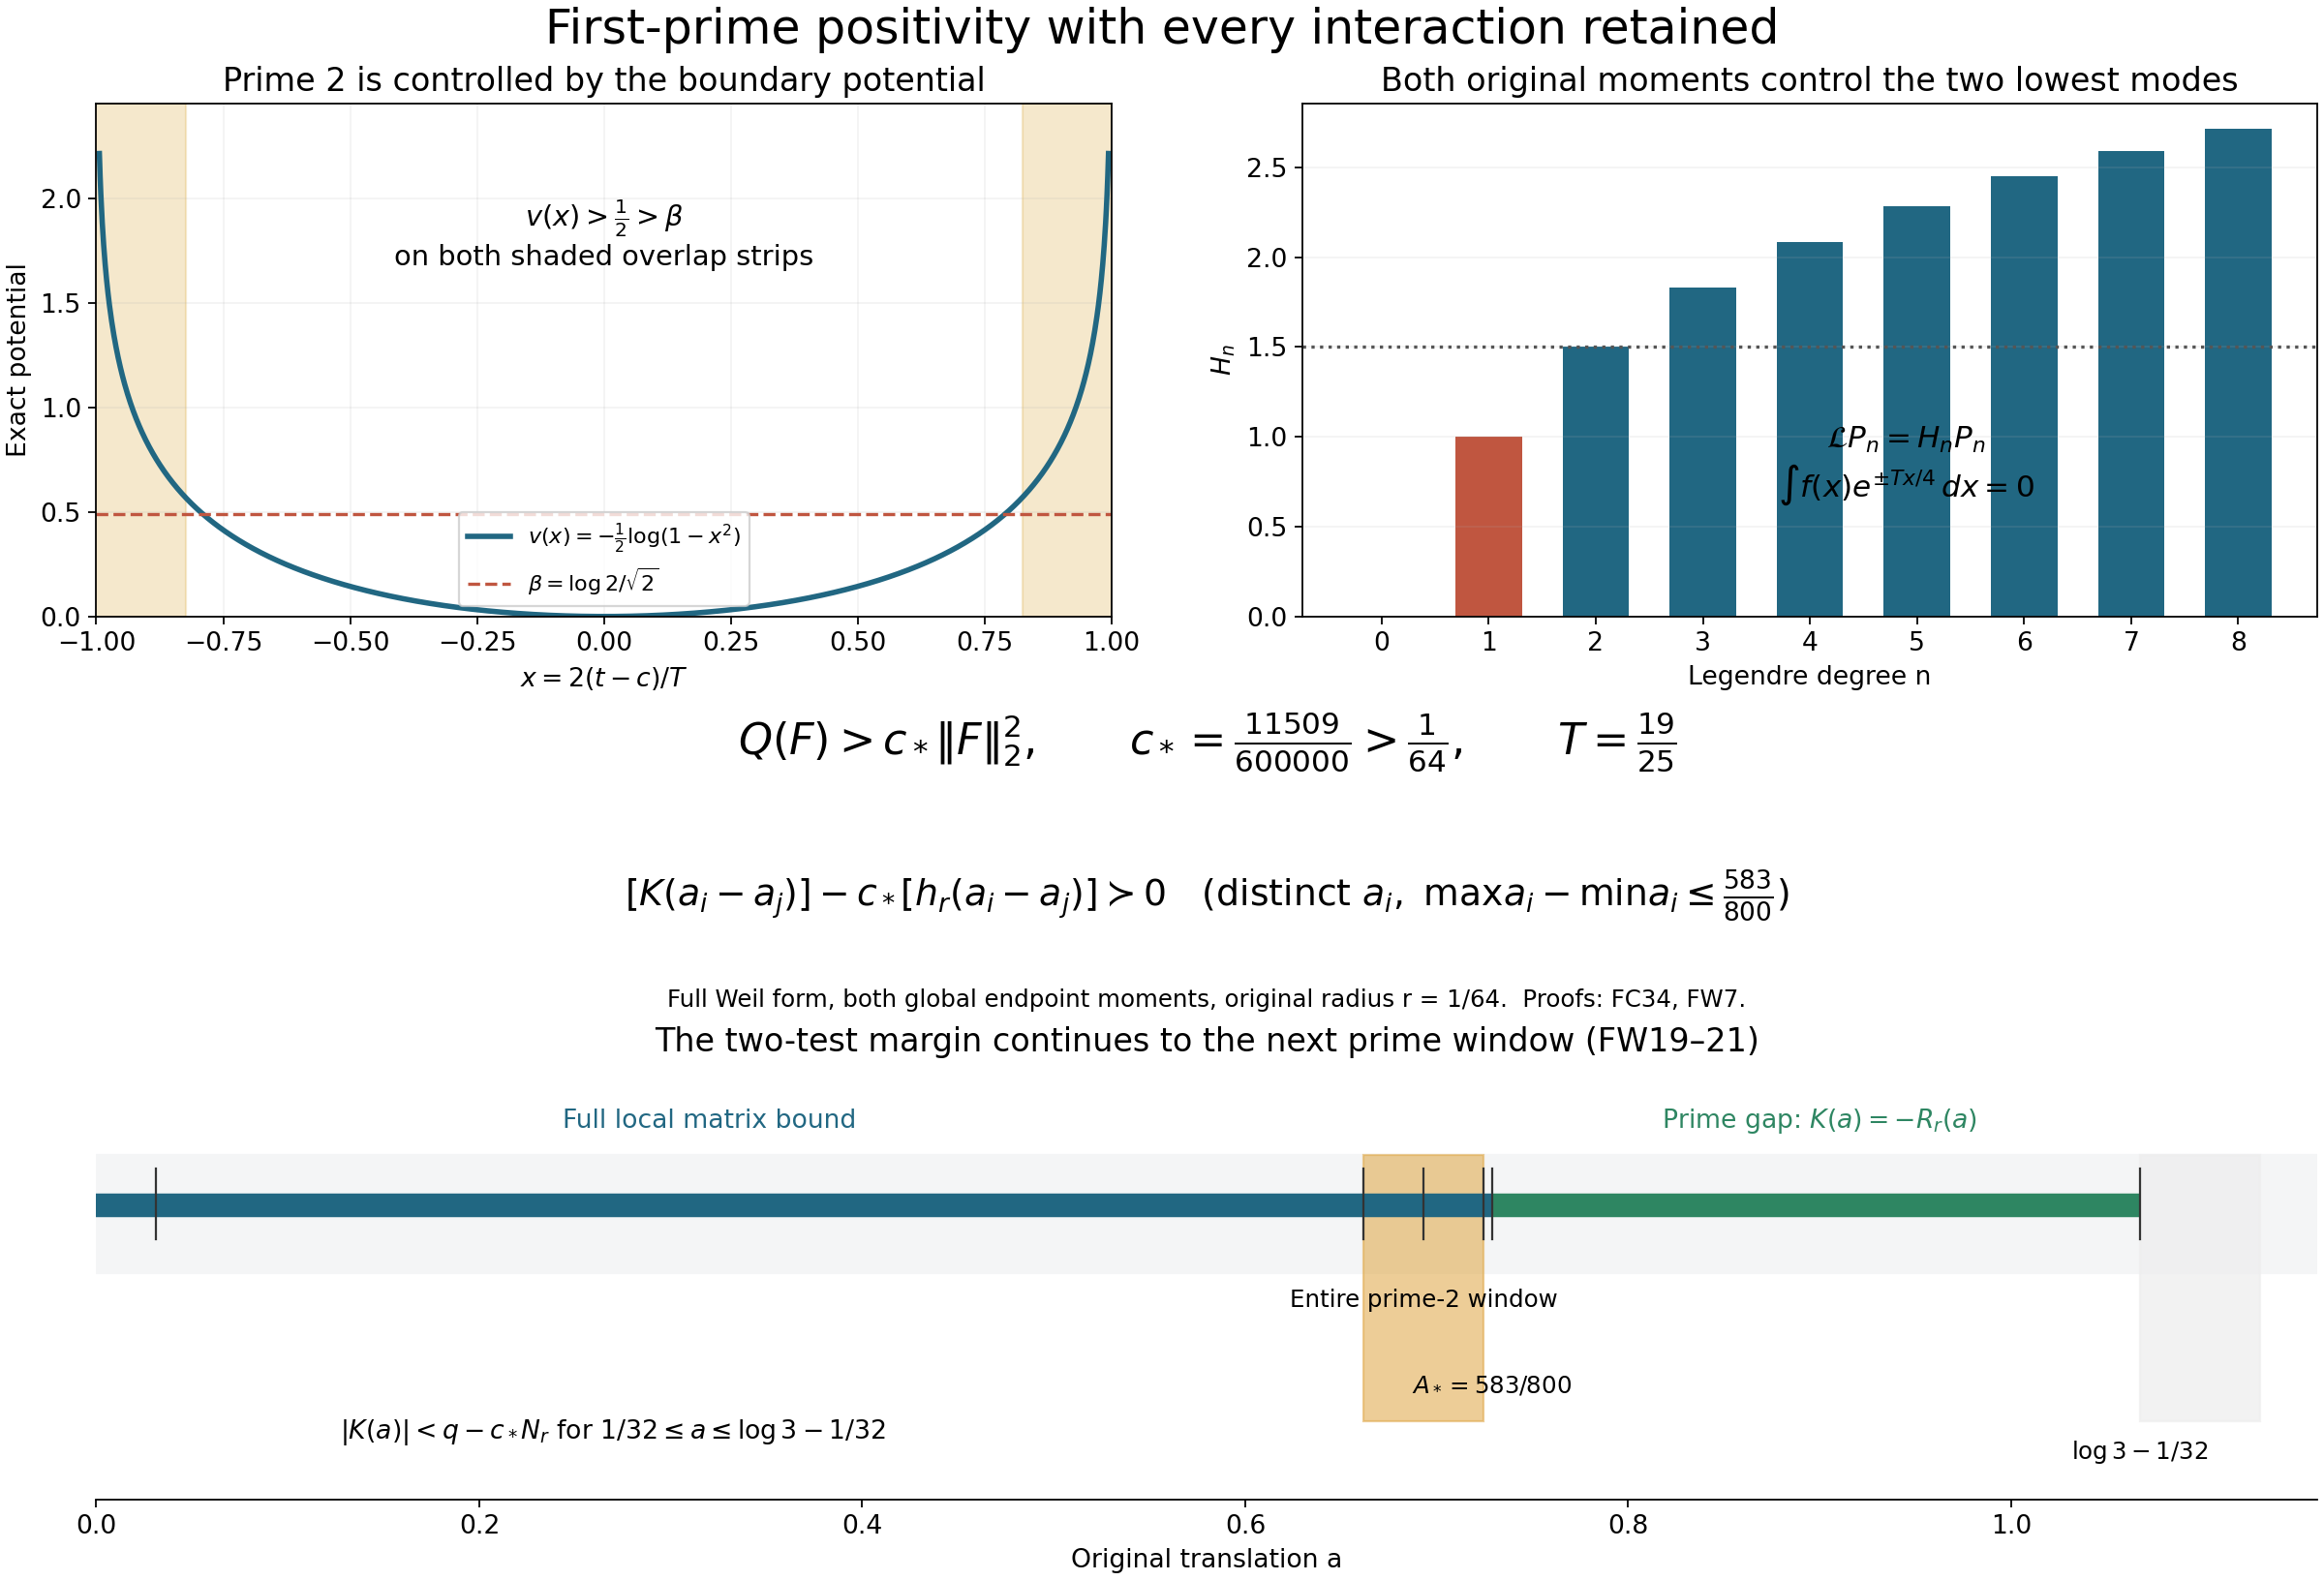
\includegraphics[keepaspectratio,alt={The full first-prime calculation. Shading shows the exact two overlap strips of the prime-2 shift in the original interval coordinate; the curve is the actual boundary potential. Harmonic-number bars show the Legendre eigenvalues, with the two global moments controlling degrees zero and one. The lower diagram gives the precise domains of the every-rank matrix bound and the longer two-test bound through the following gap. All constants, support widths and signs are those of FC19--34 and FW7--21. The classical compact density is identified with Arias de Reyna Theorem 1 by UP0. This diagram is not a plot of zeta zeros.}]{first_prime_bound.png}}
\caption{The full first-prime calculation. Shading shows the exact two
overlap strips of the prime-2 shift in the original interval coordinate;
the curve is the actual boundary potential. Harmonic-number bars show
the Legendre eigenvalues, with the two global moments controlling
degrees zero and one. The lower diagram gives the precise domains of the
every-rank matrix bound and the longer two-test bound through the
following gap. All constants, support widths and signs are those of
FC19--34 and FW7--21. The classical compact density is identified with
Arias de Reyna Theorem 1 by UP0. This diagram is not a plot of zeta
zeros.}
\end{figure}

\subsection{Proved compact-interval and finite-translation
bounds}\label{proved-compact-interval-and-finite-translation-bounds}

The complete \href{FIRST_PRIME_FULL_WEIL_COERCIVITY.md}{compact-interval
proof}, FC1--43, proves full Weil coercivity with constant 11509/600000
through support diameter 19/25, including prime 2 and both original
endpoint moments. \href{FIRST_PRIME_WINDOW_BOUND.md}{FW1--21} proves the
every-rank matrix bound for centre diameter 583/800 and a strict
two-test margin through the next prime gap. The same unchanged test now
satisfies its required strict correlation bound for every positive
translation through log 256, by
\href{FINITE_PRIME_WINDOW_EXTENSION.md}{FP1--25} and the complete
\href{FINITE_PRIME_WINDOW_COEFFICIENT_CERTIFICATE.md}{rational
prime-power certificate, FPC1--14}.
\href{PRIME_TWO_HEAT_TAIL_DERIVATION.md}{PT1--40} calculates the
surviving mixed channel and proves a strictly negative full actual right
heat derivative on the stated short interval after the prime-2 atom
ends. These are exact portions of the original bound, retaining
supported zero and every original arithmetic coefficient. The uniform
inequality beyond log 256 remains unproved.

\end{document}
